%%%%%%%%%%%%%%%%%%%%%%%%%%%%%%%%%%%%%%%%%%%%%%%%%%%
%
%  New template code for TAMU Theses and Dissertations starting Fall 2016.  
%
%
%  Author: Sean Zachary Roberson
%  Version 3.17.09
%  Last Updated: 9/21/2017
%
%%%%%%%%%%%%%%%%%%%%%%%%%%%%%%%%%%%%%%%%%%%%%%%%%%%
%%%%%%%%%%%%%%%%%%%%%%%%%%%%%%%%%%%%%%%%%%%%%%%%%%%%%%%%%%%%%%%%%%%%%%
%%                           SECTION III
%%%%%%%%%%%%%%%%%%%%%%%%%%%%%%%%%%%%%%%%%%%%%%%%%%%%%%%%%%%%%%%%%%%%%

\chapter{The LHC and CMS Detector}
\section{The Large Hadron Collider}

The Large Hadron Collider (LHC) \cite{Breskin:1244506} experiment at the European Organization for Nuclear Research (CERN) is the world's largest and most powerful particle accelerator in operation today. Located at the border between Switzerland and France, it consists of a 27-km circumference ring of superconducting magnets and accelerating structures.

Within the ring, protons are accelerated to a speed close to that of light and made to collide at 4 points:

\begin{itemize}
\item CMS (Compact Muon Solenoid) \cite{Chatrchyan:2008aa},
\item ATLAS (A Toroidal LHC ApparatuS) \cite{1748-0221-3-08-S08003},
\item ALICE (A Large Ion Collider Experiment) \cite{Aamodt:2008zz},
\item and LHCb (Large Hadron Collider beauty) \cite{Alves:2008zz}.
\end{itemize}

ATLAS and CMS are two general-purpose particle detectors located at opposite sides on the LHC ring. These are "onion-type" detectors in the sense that their general layout surrounds the interaction point with sub-detector systems aimed to measure a specific property of the particle to be detected.

The other two detectors, ALICE and LHCb are designed for specific purposes, like studying heavy-ion collisions and performing precision measurements of CP-violation and the physics of B-mesons, respectively. For this study, data collected by the CMS experiment is used.

 \begin{figure}[H]
 	\centering
 	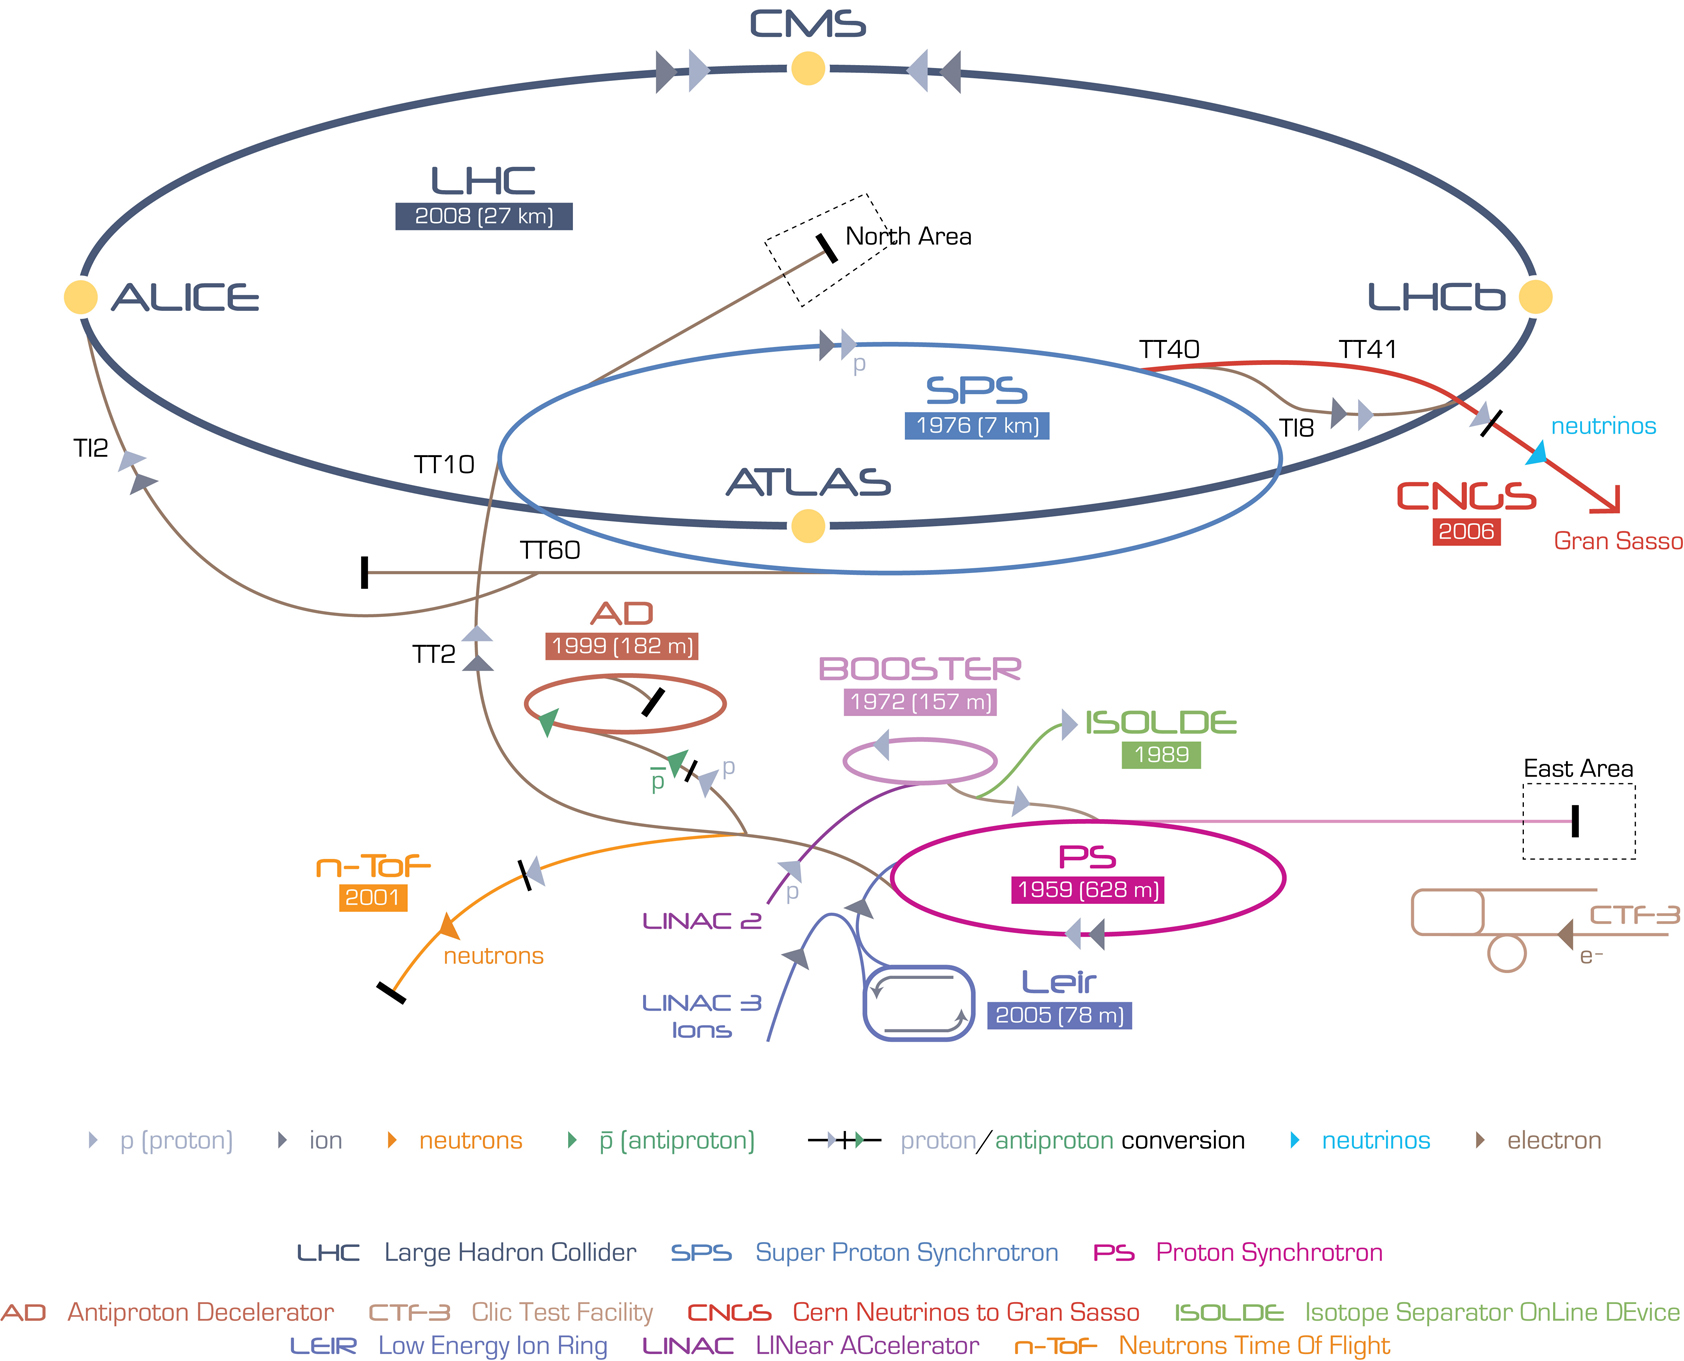
\includegraphics[width=0.75\textwidth]{figures/Cern-Accelerator-Complex.jpg}
 	\singlespace
 	\caption{Schematic diagram for the LHC experiment at CERN. Retrieved from \cite{LHC-schematic}.}
 	\label{fig:lhcdia}
 \end{figure}

 According to Einstein's famous equation $E=mc^{2}$, energy and mass are interchangeable. Therefore in order to produce heavy particles, a large amount of energy is required. The LHC was designed to produce highly energetic proton-proton, lead-proton or lead-lead beam collisions in which a variety of elementary particles can be produced.

 The beams circulating the LHC ring are not continuous streams of particles, but rather trains of regularly spaced proton bunches. The experiment was designed to operate with 2,808 bunches of protons per beam, containing about $1.5\times10^{11}$ protons per bunch separated by 25 ns, corresponding to a collision frequency of 40 MHz. 

The LHC was planned to start in September 2008, but due to an incident damaging the machine, this was not the case. The startup was delayed until November 23, 2009. Through its 2010-2011 run, the LHC operated at a center-of-mass energy of 7 TeV. Then in 2012, the energy was increased to 8 TeV, and again to 13 TeV in 2015, after a shutdown in 2013 that lasted two years.


\section{The CMS Detector}

The central feature of the CMS apparatus is a superconducting solenoid of 6 m internal diameter, providing a magnetic field of 3.8 T. The solenoidal volume contains a silicon pixel and strip tracker, a lead tungstate crystal electromagnetic calorimeter (EMCAL) and a brass and scintillator hadron calorimeter (HCAL). Each layer of the detector exploits a property of the particle to be detected to measure its energy or its momentum. 
The CMS detector was not built on site like other giant detectors of the LHC experiment, but it was constructed in 15 sections at ground level before being lowered into an underground cavern near Cessy in France and then reassembled. The complete detector is 21 m long, 12 m wide and 15 m high.

The goals of the CMS physics program range from studying the SM (including the Higgs boson) to searching for extra dimensions and dark matter. It even has a very successful heavy ion program.

The layout of the detector can be seen in Figure \ref{fig:cmsdia}. The following sections will describe each of the sub-detectors and its properties.

 \begin{figure}[H]
 	\centering
 	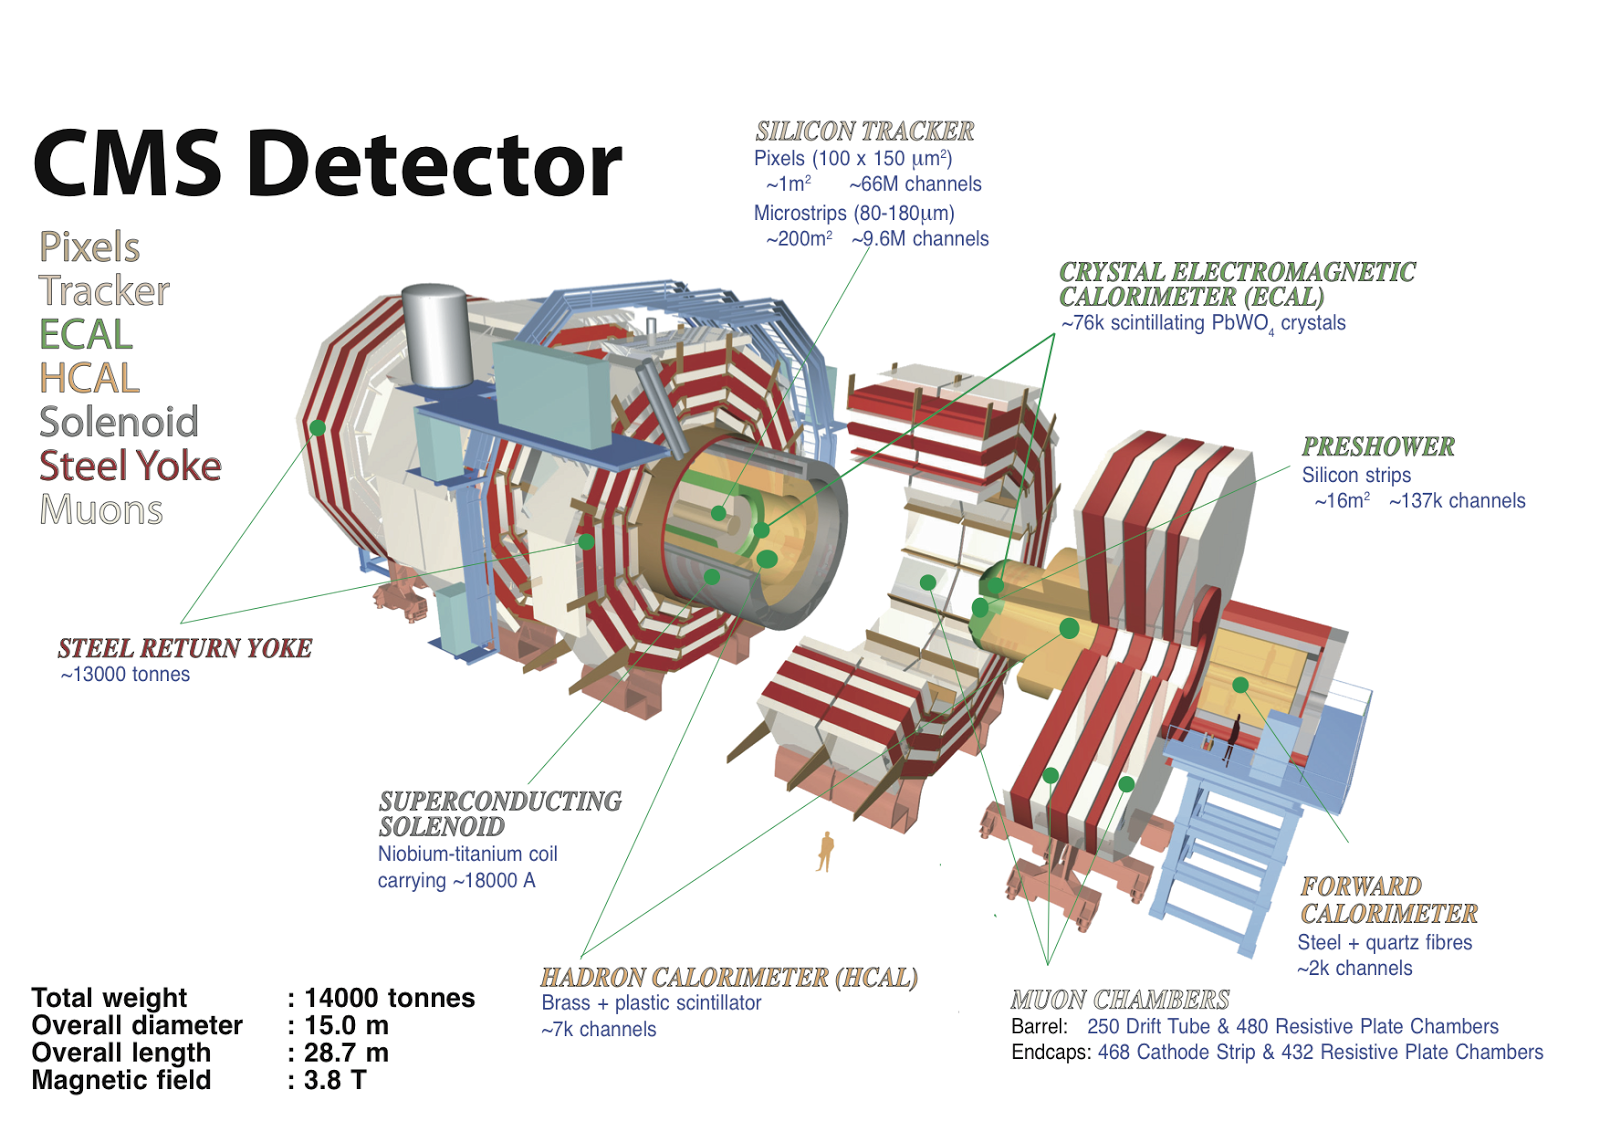
\includegraphics[width=0.85\textwidth]{figures/cms_whole.png}
 	\singlespace
 	\caption{Schematic diagram for the CMS experiment with its sub-detector systems and a person for scale. Retrieved from \cite{CMS-schematic}.}
 	\label{fig:cmsdia}
 \end{figure}

 \subsection{Coordinate System}

 The CMS experiment uses a right-handed coordinate system, with the origin at the nominal collision point, the $x$-axis pointing to the center of the LHC ring, the $y$-axis pointing up (perpendicular to the LHC plane), and the $z$-axis along the anticlockwise beam direction. The polar angle $\theta$ is measured from the positive $z-axis$ and the azimuthal angle $\phi$ is measured from the positive $x$-axis in the $x-y$ plane. The radius $r$ denotes the distance from the $z$-axis and the pseudorapidity $\eta$ is defined as $\eta=-log[tan(\theta \ 2)]$. $\eta$ is preferently used by CMS particle physicists to measure forward-ness of relativistic particles in the detector since any differences in this coordinate are invariant under boosts in the $z-$direction and particle production is roughly uniform in $\eta$. See Figure \ref{fig:cmscor} for reference.

  \begin{figure}[H]
 	\centering
 	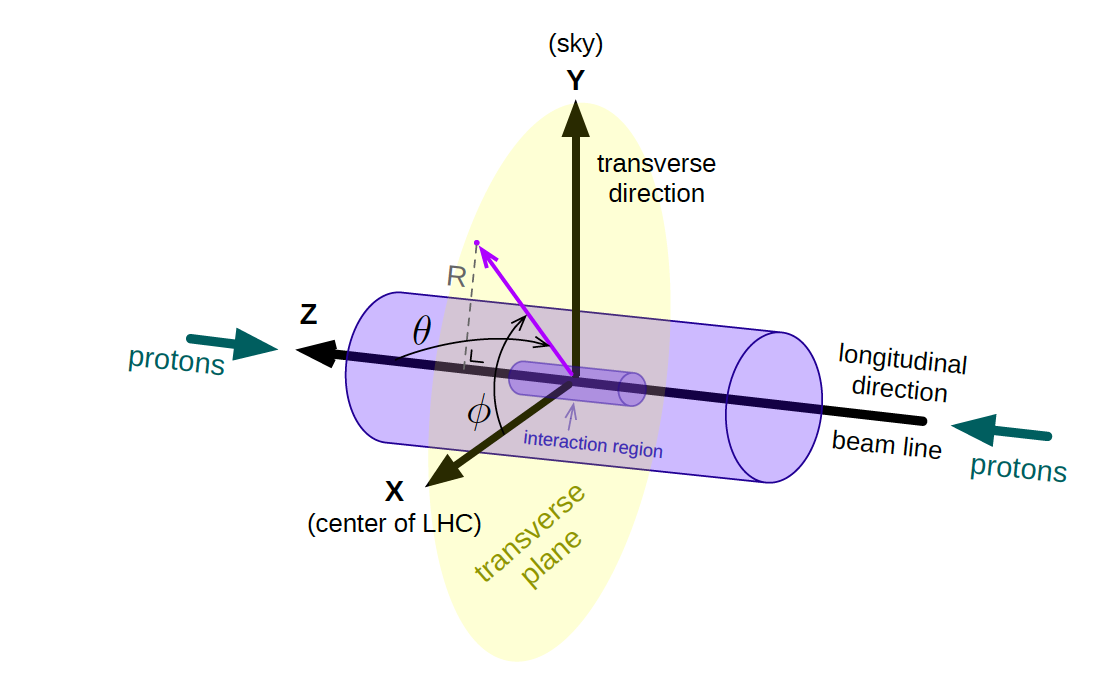
\includegraphics[width=0.5\textwidth]{figures/corsyslhc.png}
 	\singlespace
 	\caption{Diagram for the CMS detector coordinate system.}
 	\label{fig:cmscor}
 \end{figure}

 \subsection{Tracker and Pixel Detector}
 Momentum analysis in CMS makes use of the magnetic field provided by its super-conducting solenoid. The tracker sub-detector is not only able to measure the momentum of charged particles but also determines their direction at their production vertex.

 The full sillicon inner tracking system\cite{trackeradd} is a cylinder-shaped detector with an outer radius of 1.2 m and a length of 5.6 m. The barrel(each of the two endcaps) includes three(two) layers of pixel detectors, surrounded by ten(twelve) layers of micro-strip detectors. The 16,588 silicon sensor moduels are finely segmented into 66 million 150$\times$100 $\mu$m pixels and 9.6 million 80-to180 $\mu$m-wide strips. Figure \ref{fig:cmstracker} shows the layout of the tracker and its subsystems.

   \begin{figure}[H]
 	\centering
 	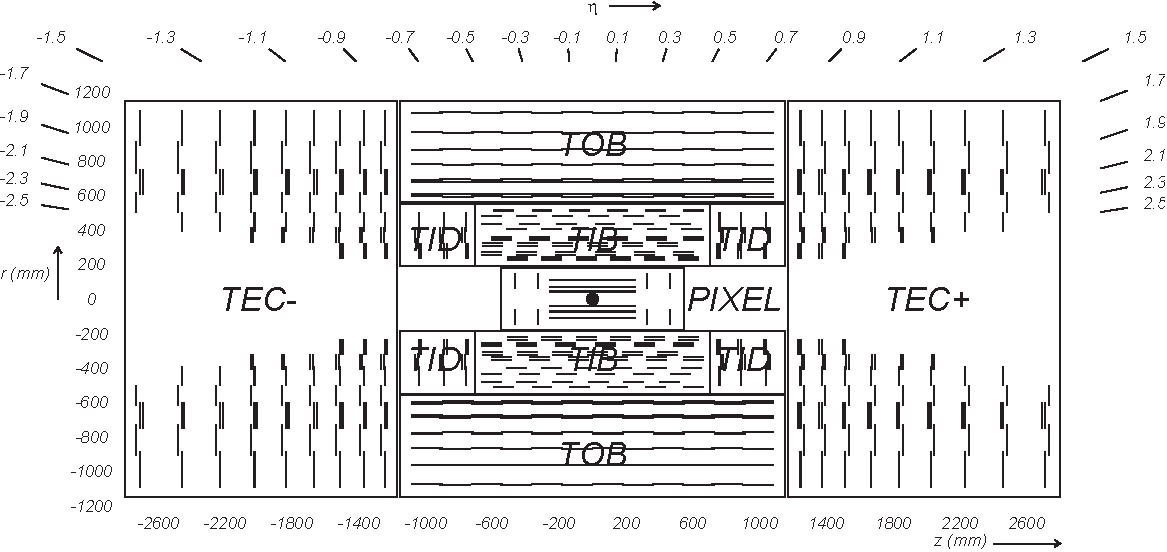
\includegraphics[width=0.9\textwidth]{figures/CMS_tracker.pdf}
 	\singlespace
 	\caption{Layout of the CMS detector tracker with subsystems labeled.}
 	\label{fig:cmstracker}
 \end{figure}

The pixel detector is made up of three barrel layers, called BPIX, and two endcap layers called the FPIX. The BPIX contains 48 million pixels and the FPIX contains another 18 million pixels. In total it consists of 1440 hybrid silicon detector modules, each with a dimension of $100 \times 150 \mu m^{2}$. The small pixel size enables track resolutions of 10$\mu m$ in the transverse plane and 20$\mu m$ in the $z$-direction. The pixel detector is what gives CMS its excellent secondary vertex tagging ability in addition to producing seed tracks for the strip tracker and the high level trigger (HLT).

Likewise, the silicon strip detector is made up of four subsystems. The Tracker Inner Barrel (TIB) has four layers of 320 $\mu m$ strips. At each end of the TIB is a three-layer Tracker Inner Disks (TID), which contains strips of the same thickness. The Tracker Outer Barrel (TOB) is the six layer system which surrounds the TIB/TID. The first four layers of the TOB use 500$\mu m$ thick strips, and the last two layers use 122 $\mu m$ thick strips. The Tracker EndCaps (TEC) are on either side of the previous setup and contain nine disks with up to seven layers of strips. These strips are 320 $\mu m$ thick in the inner four rings and 500 $\mu m$ in the outer three rings. In total, the strip detector contains 9.3 million silicon strips.

The tracker measures the $p_{T}$ of charged hadrons at normal incidence with a resolution of 1$\%$ for $p_{T}<$ 20 GeV\cite{Sirunyan_2017}. The relative resolution then degrades with increasing $p_{T}$ to reach the calorimeter energy resolution for track momenta of several hundred GeV.

 \subsection{Electromagnetic Calorimeter}

 The CMS ECAL\cite{CERN-LHCC-97-033} is a homogeneous calorimeter made out of lead tungstate ($PbWO_{4}$) crystals totaling 75,848 units. The detector is divided up into two sections which provide a coverage of $|\eta| < 1.479$ in the barrel region (EB) and $1.479 < |\theta| < 3.0$ in two endcap regions (EE). There are also preshower detectors (PS) in each of the endcaps, in fornt of the EE, which cover a pseudorapidity range of $1.653 < |\eta| < 2.6$. Figure \ref{fig:cmsecal} shows the structure of the ECAL.

    \begin{figure}[H]
 	\centering
 	\includegraphics[width=0.9\textwidth]{figures/ECAL_transverse_Section.pdf}
 	\singlespace
 	\caption{A schematic of the CMS ECAL detector with its subsystems labeled.}
 	\label{fig:cmsecal}
	 \end{figure}

Each calorimeter cristal has a depth of 230 mm, which corresponds to 25.8 radiation lengths ($X_{0}$) for $PbWO_{4}$, sufficient to contain more than 98$\%$ of the energy of electrons and photont up to 1 TeV. The scintillation light produced in the crystals is read out by avalanche photodiodes (APDs), which produce approximately 4.5 photoelectrons per MeV at room temperature. 

The crystal transverse size matches the small Moliére radius of $PbWO_{4}$, 2.2 cm. This fine transverse granularity makes it possible to fully resolve hadron and photon energy deposits as close as 5 cm from one another.

The intrinsic energy resolution ($\sigma$) of the ECAL barrel was measured with an ECAL supermodule directly exposed to an electron beam\cite{Ingram_2007}. The relative energy resolution is typically parameterized as a function of the electron energy as

\begin{equation}
\frac{\sigma_{E}}{E} = \frac{2.8\%}{E[GeV]} \oplus \frac{12\%}{\sqrt{E[GeV]}} \oplus 0.3\%
\end{equation}

 \subsection{Hadron Calorimeter}

 The CMS HCAL\cite{CMS:1997tfa} is a sampling calorimeter, meaning it finds a particle's position, energy and arrival time using alternating layers of "absorber" and fluorescent scintillator or "active" materials that produce a rapid light pulse when the particle passes through.The produced light is then collected by optic fibers that feed it into readout boxes where photodetectors amplify the signal. The amount of light in a given region is summed up over many layers of tiles in depth, called a "tower". 

 The HCAL is organized into barrel (HB and HO), endcap (HE), and forward (HF). There are 36 barrel "wedges", each weighting 26 tonnes. These form the last layer of detector inside the magnetic coil. A few additional layers, the outer barrel (HO), sit outside the coil, ensuring no energy leaks out the back of the HB undetected. Similarly, 36 endcap wedges measure particle energies as they emerge through the ends of the solenoid magnet. In the barrel, the HCAL absorber thickness amounts to almost six interaction lengths at normal incidence, and increases to over ten interaction lengths at larger pseudorapidities. The HO material corresponds to 1.4 interaction lengths at normal incidence.

 Lastly, the two hadronic forward calorimeters (HF) are positioned at either end of CMS, to detect particles coming out of the collision region at shallow angles relative to the beam line. These receive the bulk of the particle energy contained in the collision so must be very radiation resistant. Figure \ref{fig:cmshcal} shows the structure and position of the HCAL subsystems. 

     \begin{figure}[h]
 	\centering
 	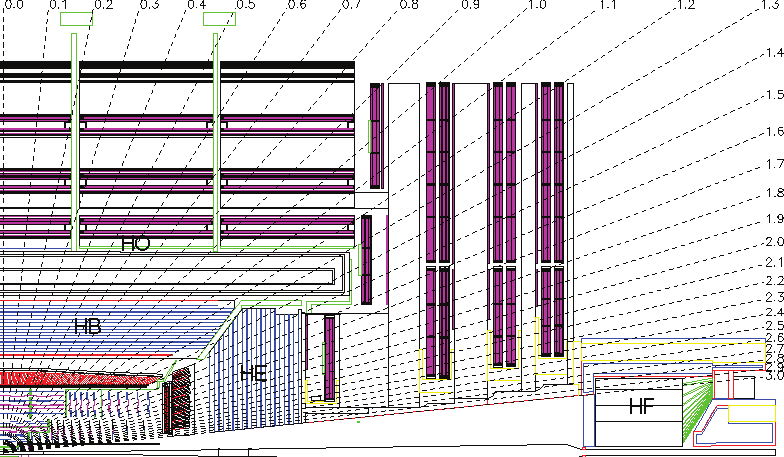
\includegraphics[width=0.9\textwidth]{figures/HCAL_subdet.pdf}
 	\singlespace
 	\caption{Structure and position of the CMS HCAL sub-detector systems.}
 	\label{fig:cmshcal}
	 \end{figure}

Combined, the ECAL and HCAL can measure the energy deposited by a charged pion with a resolution of $\sigma/E\approx100\%/\sqrt{E[GeV]}\oplus5\%$ \cite{Yazgan_2009}, assuming an average jet particle composition.

 \subsection{Solenoid}

 The CMS magnet\cite{Acquistapace:1997fm} is the central device around which the experiment is built. It delivers a 4T magnetic field, which is 100,000 times stronger than that of Earth over a length of 12.5 m and a free-bore radius of 3.15 m.

 Its job is to bend the paths of charged particles emerging from high-energy collisions in the LHC. The higher momentum particles get their path curved less than the lighter ones, and as a result, curvature is an important tool for momentum measurements. 

 The strong magnetic field, combined with the high-precision position measurements in the tracker and muon detectors, allows for accurate measurement of the momentum of high-energy particles.

 The CMS solenoid magnet is made of coils of wire that produce a uniform magnetic field when electricity flows through them. Also, it is superconducting, the largest ever built, with a weight of 12,000 tonnes. In order for it to be superconducting, it needs to be colled down to -268.5 C, which is a degree warmer than outer space.

 The tracker and calorimeter detectors fit inside the magnet while the muon detectors are interleaved with a 12-sided iron structure that surrounds the magnet coils and contains and guides the field. Made up of three layers, this "return yoke" reaches out 14 meters in diameter and also acts as a filter, allowing through only muons and weakly interacting particles such as neutrinos. The enormous magnet also provides most of the experiment's structural support, and must be very strong itself to withstand the forces of its own magnetic field.


 \subsection{Muon System}
 After its magnet, the main feature of the CMS experiment is its capability of detecting muons. Since they can penetrate several meters of iron without interacting, gas-ionization detector chambers were placed at the very edge of the experiment embedded in the steel flux-return yoke in order to detect them. This allows for a pseudorapidity coverage of $|\eta| < 2.4$.

 The muon system consists of 1400 muon chambers which can be classified into three categories, according to the technology used: 250 drift tubes (DTs), 540 cathode strip chambers(CSCs), and 610 resistive plate chambers(RPCs).

 The barrel region of the detector contains DT's and RPCs, while the endcap region contains CSCs and RPCs. The layout of the muon system can be seen in Figure \ref{fig:cmsmuonsys}. 

    \begin{figure}[h]
 	\centering
 	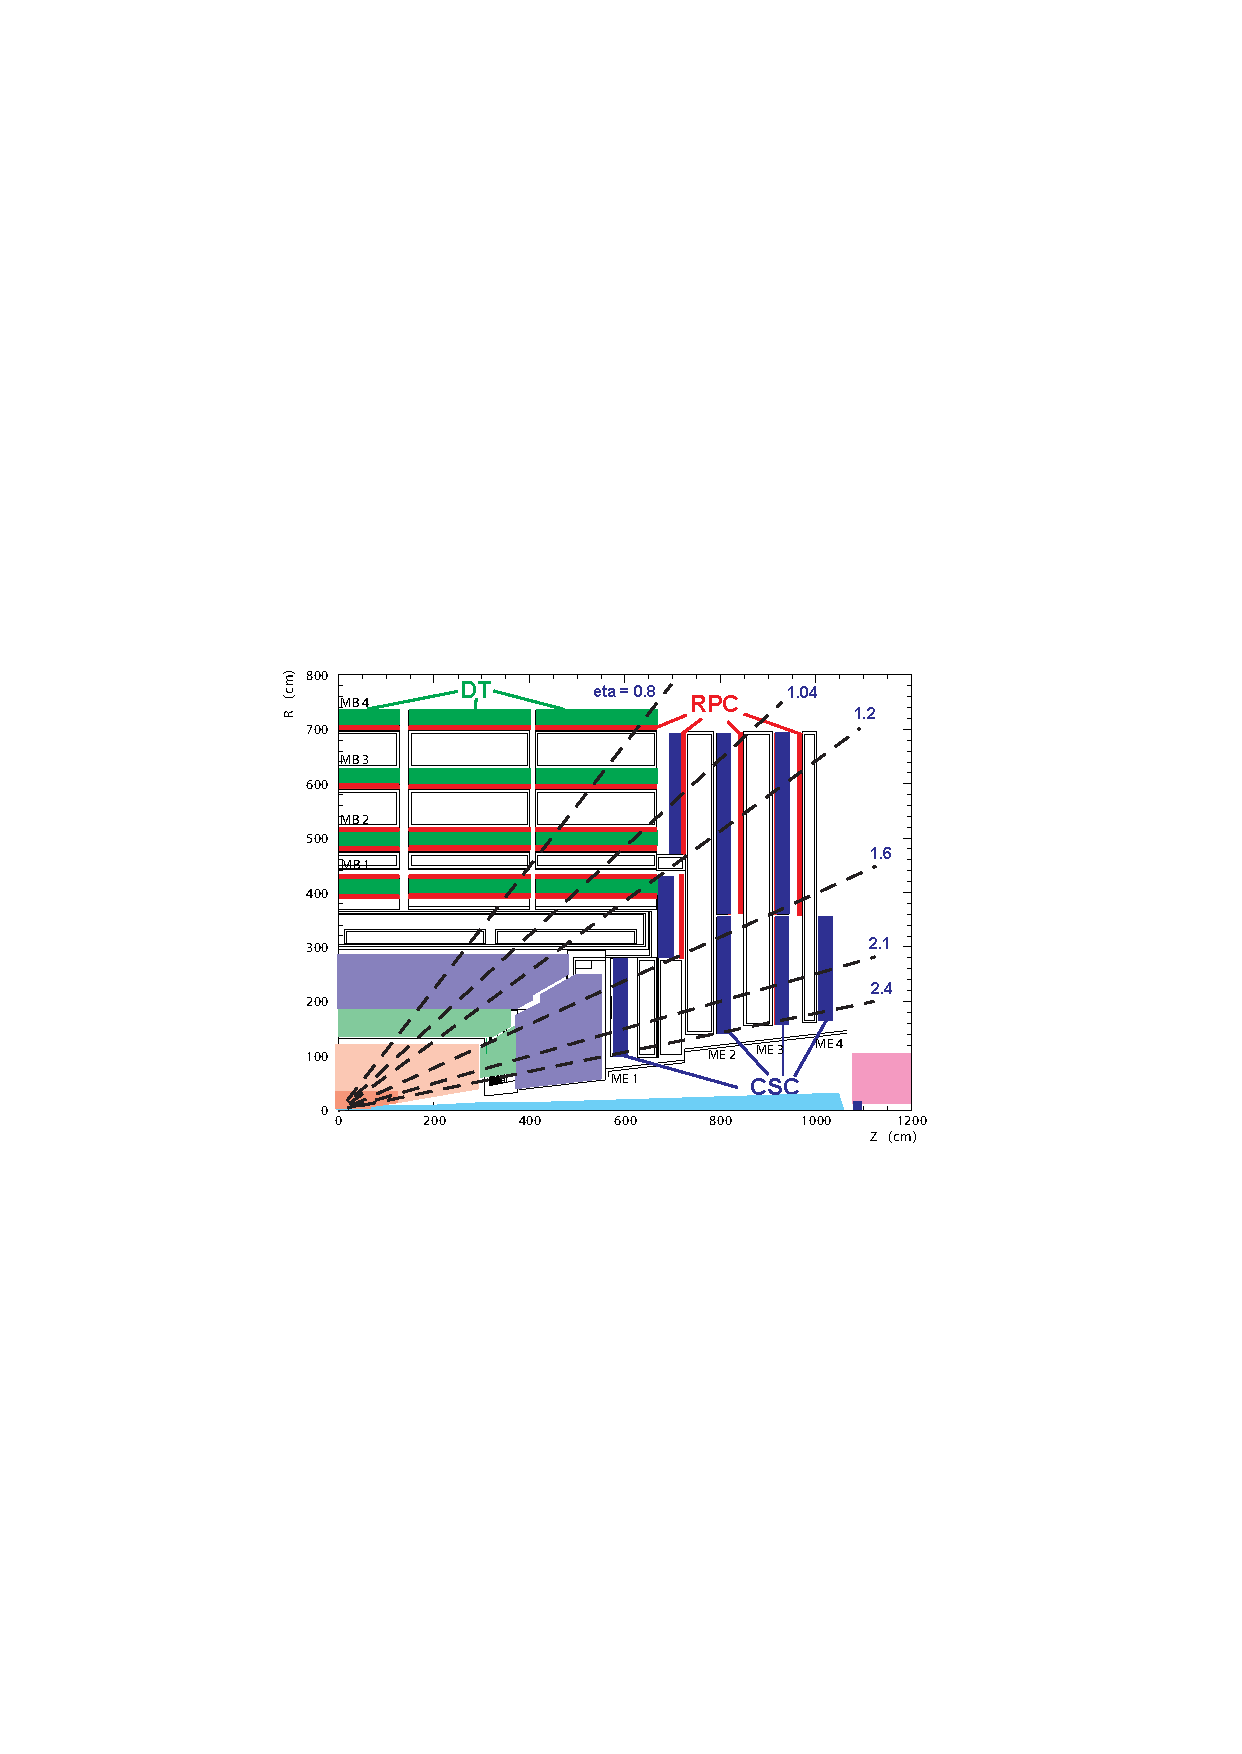
\includegraphics[width=0.9\textwidth]{figures/CMS_muon_system.pdf}
 	\singlespace
 	\caption{Layout of the CMS muon system.}
 	\label{fig:cmsmuonsys}
	\end{figure}

The four muon DT stations sitting outside the magnet coil are interleaved with the
iron "return yoke" (shown in red in Figure \ref{fig:cmsmuchambers}, for the barrel region), which not only returns the flux from the solenoid, but also shields the muon chambers from hadrons. 

    \begin{figure}[h]
 	\centering
 	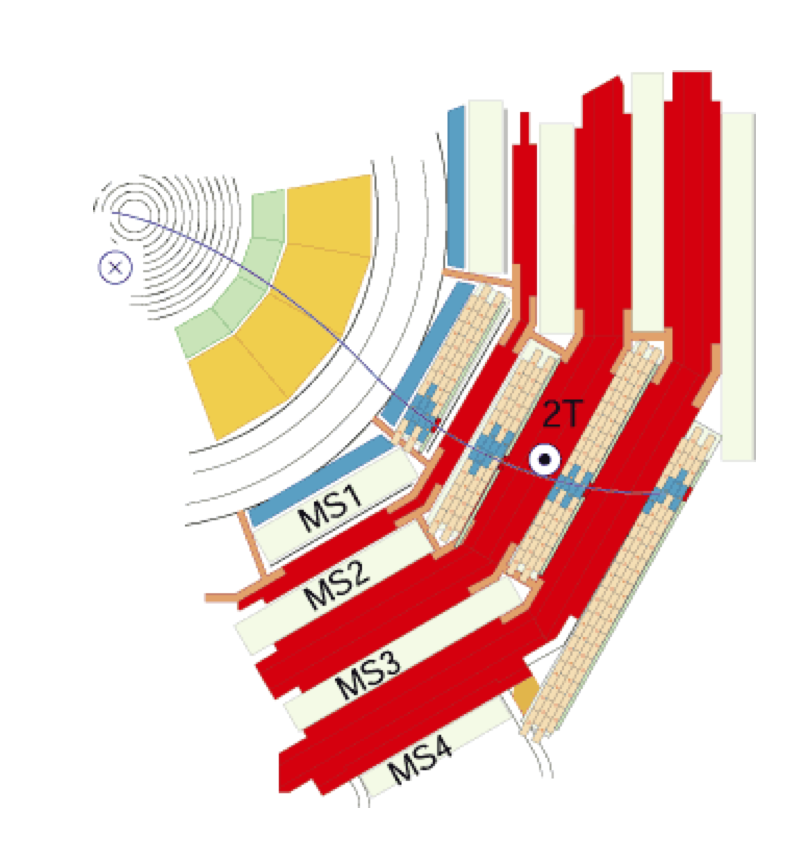
\includegraphics[width=0.5\textwidth]{figures/MuStations.png}
 	\singlespace
 	\caption{A muon, in the plane perpendicular to the LHC beams, leaves a curved trajectory in four layers of muon detectors or stations.}
 	\label{fig:cmsmuchambers}
	\end{figure}

The CSCs track the particle's position and allow for triggering, while the RPCs form a redundant trigger system, which quickly decides to keep the acquired muon data or not. Because of the many layers of detector and different specialties of each type, the system is naturally robust and able to filter out background noise.

The muon system on its own has a resolution of 15-40$\%$ depending on $\eta$. Matching muons to tracks measured in the silicon tracker results in a relative transverse momentum resolution for muons with 20$< p_{T} < $ 100 GeV of 1.3-2.0$\%$ in the barrel and better than 6$\%$ in the endcaps. The $p_{T}$ resolution in the barrel is better than 10$\%$ for muons up to 1 TeV \cite{Chatrchyan:2012xi}.

\subsection{Luminosity Measurement}

The two most important features of a particle accelerator are its center of mass energy and its instantaneous luminosity ($\mathcal{L}$). The latter provides a measurement of the number of collisions that can be produced in the accelerator per squared centimeter and per second.

Besides measuring the kinematics of each of the particles traversing the detector, CMS must also measure the instantaneous luminosity delivered by the LHC. Both the pixel detector, and the HF are able to measure the luminosity to varying degrees of accuracy.

For a given process, the number of interactions (N) is the product of $\mathcal{L}$ integrated over the data taking time period and the cross section for the process in question ($\sigma_{ref}$):

\begin{equation}
N = \sigma_{ref}\int\mathcal{L}(t)dt
\end{equation} 


The Van der Meer (VdM) scan method measures the size and shape of the interaction region of the colliding beams. This is achieved by displacing the beams in the x and y- (transverse) planes and measuring the relative interaction rates as a function of the transverse beam separation. For Gaussian beams, the luminosity as a function of the transverse displacement ($\delta u$) can then be expressed as:  

\begin{equation}
\mathcal{L}(\delta u) = \mathcal{L}_{0} exp[-\frac{\delta u^{2}}{2\sigma_{u}^{2}}]
\end{equation}

where 

\begin{equation}
\mathcal{L}_{0} = \frac{N_{1}N_{2}fN_{b}}{2\pi\sqrt{(\sigma_{1x}^{2}+\sigma_{2x}^{2})(\sigma_{1y}^{2}+\sigma_{2y}^{2})}}
\end{equation}

and $\sigma_{u} = \sqrt{\sigma_{1u}^{2}+\sigma_{2x}^{2}}$ with $u=x,y$ for each separation plane, $N_{b}$ the number of colliding bunches and $f$ the revolution frequency.

A fit of the measured interaction rates as a function of the reparation will allow to determine the effective beam size as well as the maximum achievable collision rate ($\dot{N}$)

\begin{equation}
\dot{N} = \mathcal{L}\sigma
\end{equation}

In practice, the scans are performed by moving the beams step-wise across each other in the two transverse plane.

% Notice that the title of this section is long - much longer than the others. When you have long section titles, this template takes care of double spacing the lines in the title. If the title is long to fit in the table of contents, the template will single space the title.

% \section{Yet Another Table}

% Another table is placed here to show the effect of having tables in multiple sections. The list of tables should still double space between table titles, while single spacing long table titles.

% %Fix table labeling.
% \begin{table}[h!]
% 	\centering
% 	\begin{tabular}{|l|l|}
% 		\hline
% 		Dates & Attendance  \\ \hline
% 		August 8-10, 2008 & 3,523  \\ \hline
% 		August 14-16, 2009 & 4,003 \\ \hline
% 		July 9-11, 2010 & 5,049 \\ \hline
% 		August 5-7, 2011 & 6,891  \\ \hline
% 		August 10-12, 2012 & 9,464  \\ \hline
% 		August 16-18, 2013 & 11,077  \\ \hline
% 		July 18-20, 2014 & 14,686 \\ \hline
% 		July 31-August 2, 2015 & 18,411  \\ \hline
% 	\end{tabular}
% 	\caption{San Japan attendance. Data is taken from \cite{ANCONS}. I intentionally make the title of this table long so the single space effect is seen in the list of tables.}
% \end{table}

% You may be wondering why San Japan was chosen. There are a few reasons as to why I did this:

% \begin{enumerate}
% \item It is one of the fastest-growing anime conventions in Texas.
% \item Filler.
% \item I wanted a good variety of table examples.
% \item Because conventions are cool.
% \end{enumerate}

% The \textit{enumerate} environment was used to generated an ordered list above.

% \section{Section Test Example}
% We insert another figure here, just for kicks.

% \begin{figure}[h!]
% 	\centering
% 	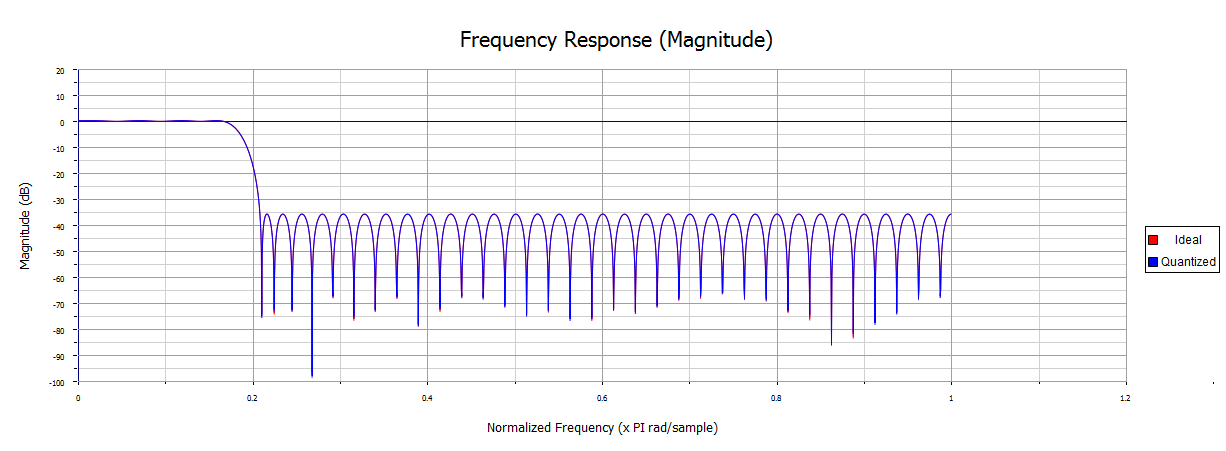
\includegraphics[width = 6.0in]{LowPass_Filter_Design.png}
% 	\caption{A low pass filter design.}
% \end{figure}

% \subsection{Filler, Filler, Filler}

% This section has filler text. These words serve no meaning except to fill a few lines in the document. This section has filler text. These words serve no meaning except to fill a few lines in the document. This section has filler text. These words serve no meaning except to fill a few lines in the document.

% \begin{figure}[h!]
% 	\centering
% 	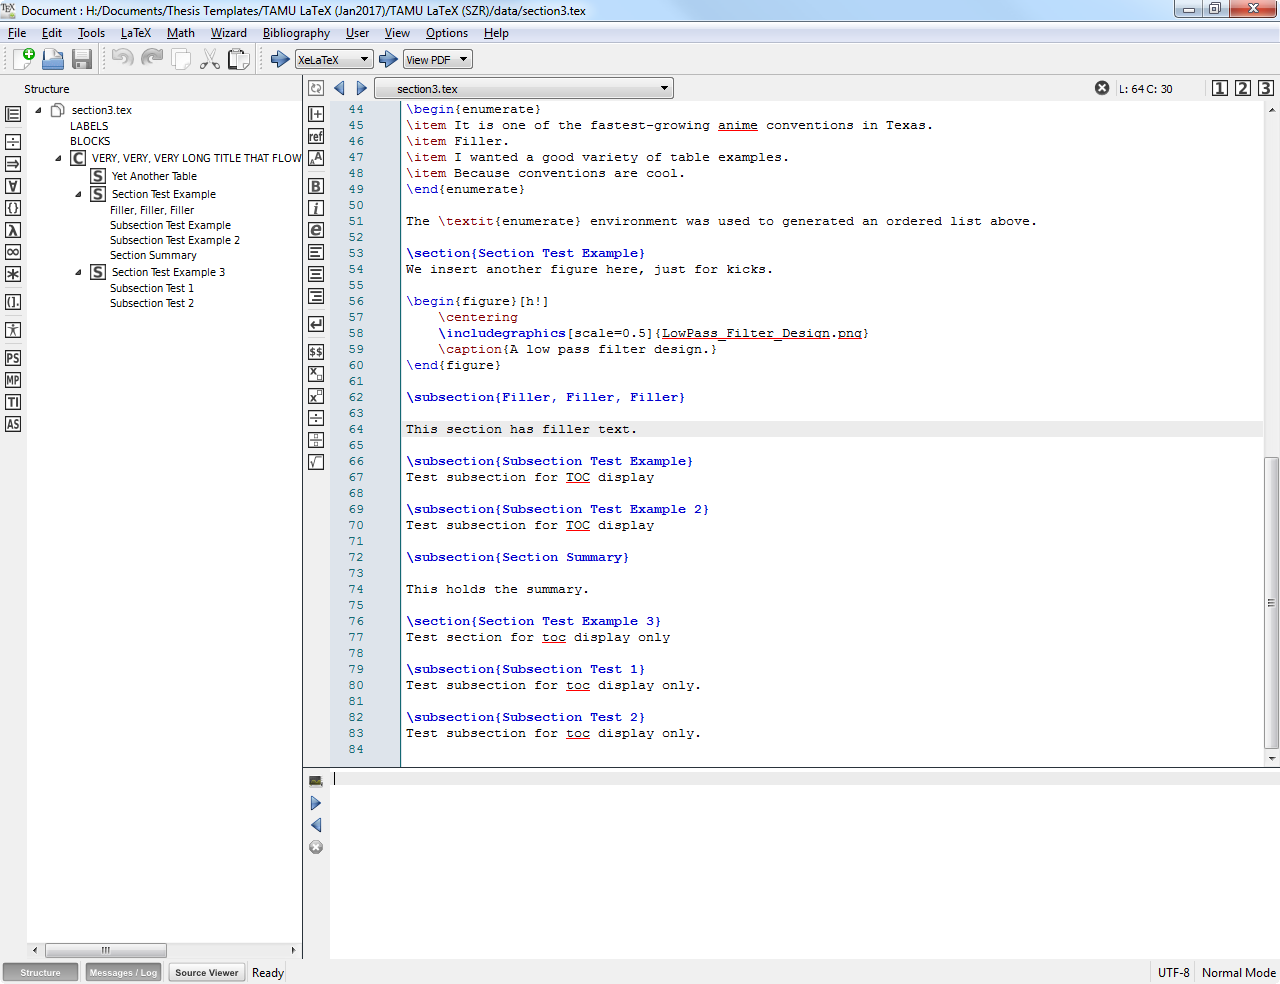
\includegraphics[width=3.75in]{Workspace1.png}
% 	\caption{A typical Texmaker workspace in Windows 7. The right sidebar displays the current file's structure according to the subsections in place.}
% \end{figure}

% This section has filler text. These words serve no meaning except to fill a few lines in the document. This section has filler text. These words serve no meaning except to fill a few lines in the document. This section has filler text. These words serve no meaning except to fill a few lines in the document. This section has filler text. These words serve no meaning except to fill a few lines in the document. This section has filler text. These words serve no meaning except to fill a few lines in the document. This section has filler text. These words serve no meaning except to fill a few lines in the document.

% \begin{figure}[h!]
% 	\centering
% 	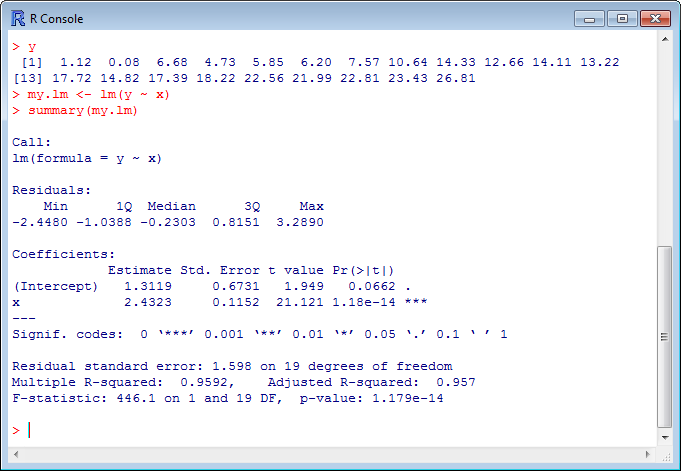
\includegraphics[width=3.5in]{Rachl1.png}
% 	\caption{Some commands in R.}
% \end{figure}

% \subsection{Subsection Test Example}
% Test subsection for TOC display

% \subsection{Subsection Test Example 2}
% This section has filler text. These words serve no meaning except to fill a few lines in the document. This section has filler text. These words serve no meaning except to fill a few lines in the document. This section has filler text. These words serve no meaning except to fill a few lines in the document.

% \begin{figure}[h!]
% 	\centering
% 	
\includegraphics[scale=0.85]{TAM_Logo1.png}
% 	\caption{The logo of a familiar university.}
% \end{figure}

% \begin{figure}[!h]
% 	\caption{Yet another blank float that has no purpose. This is only to test the appearance of the Lists of Figures and the List of Tables.}
% \end{figure}

% \subsection{Section Summary}
  
% This holds the summary. Well, not really a summary - there was a lot of filler in this section.

% \begin{figure}[h!]
% 	\centering
% 	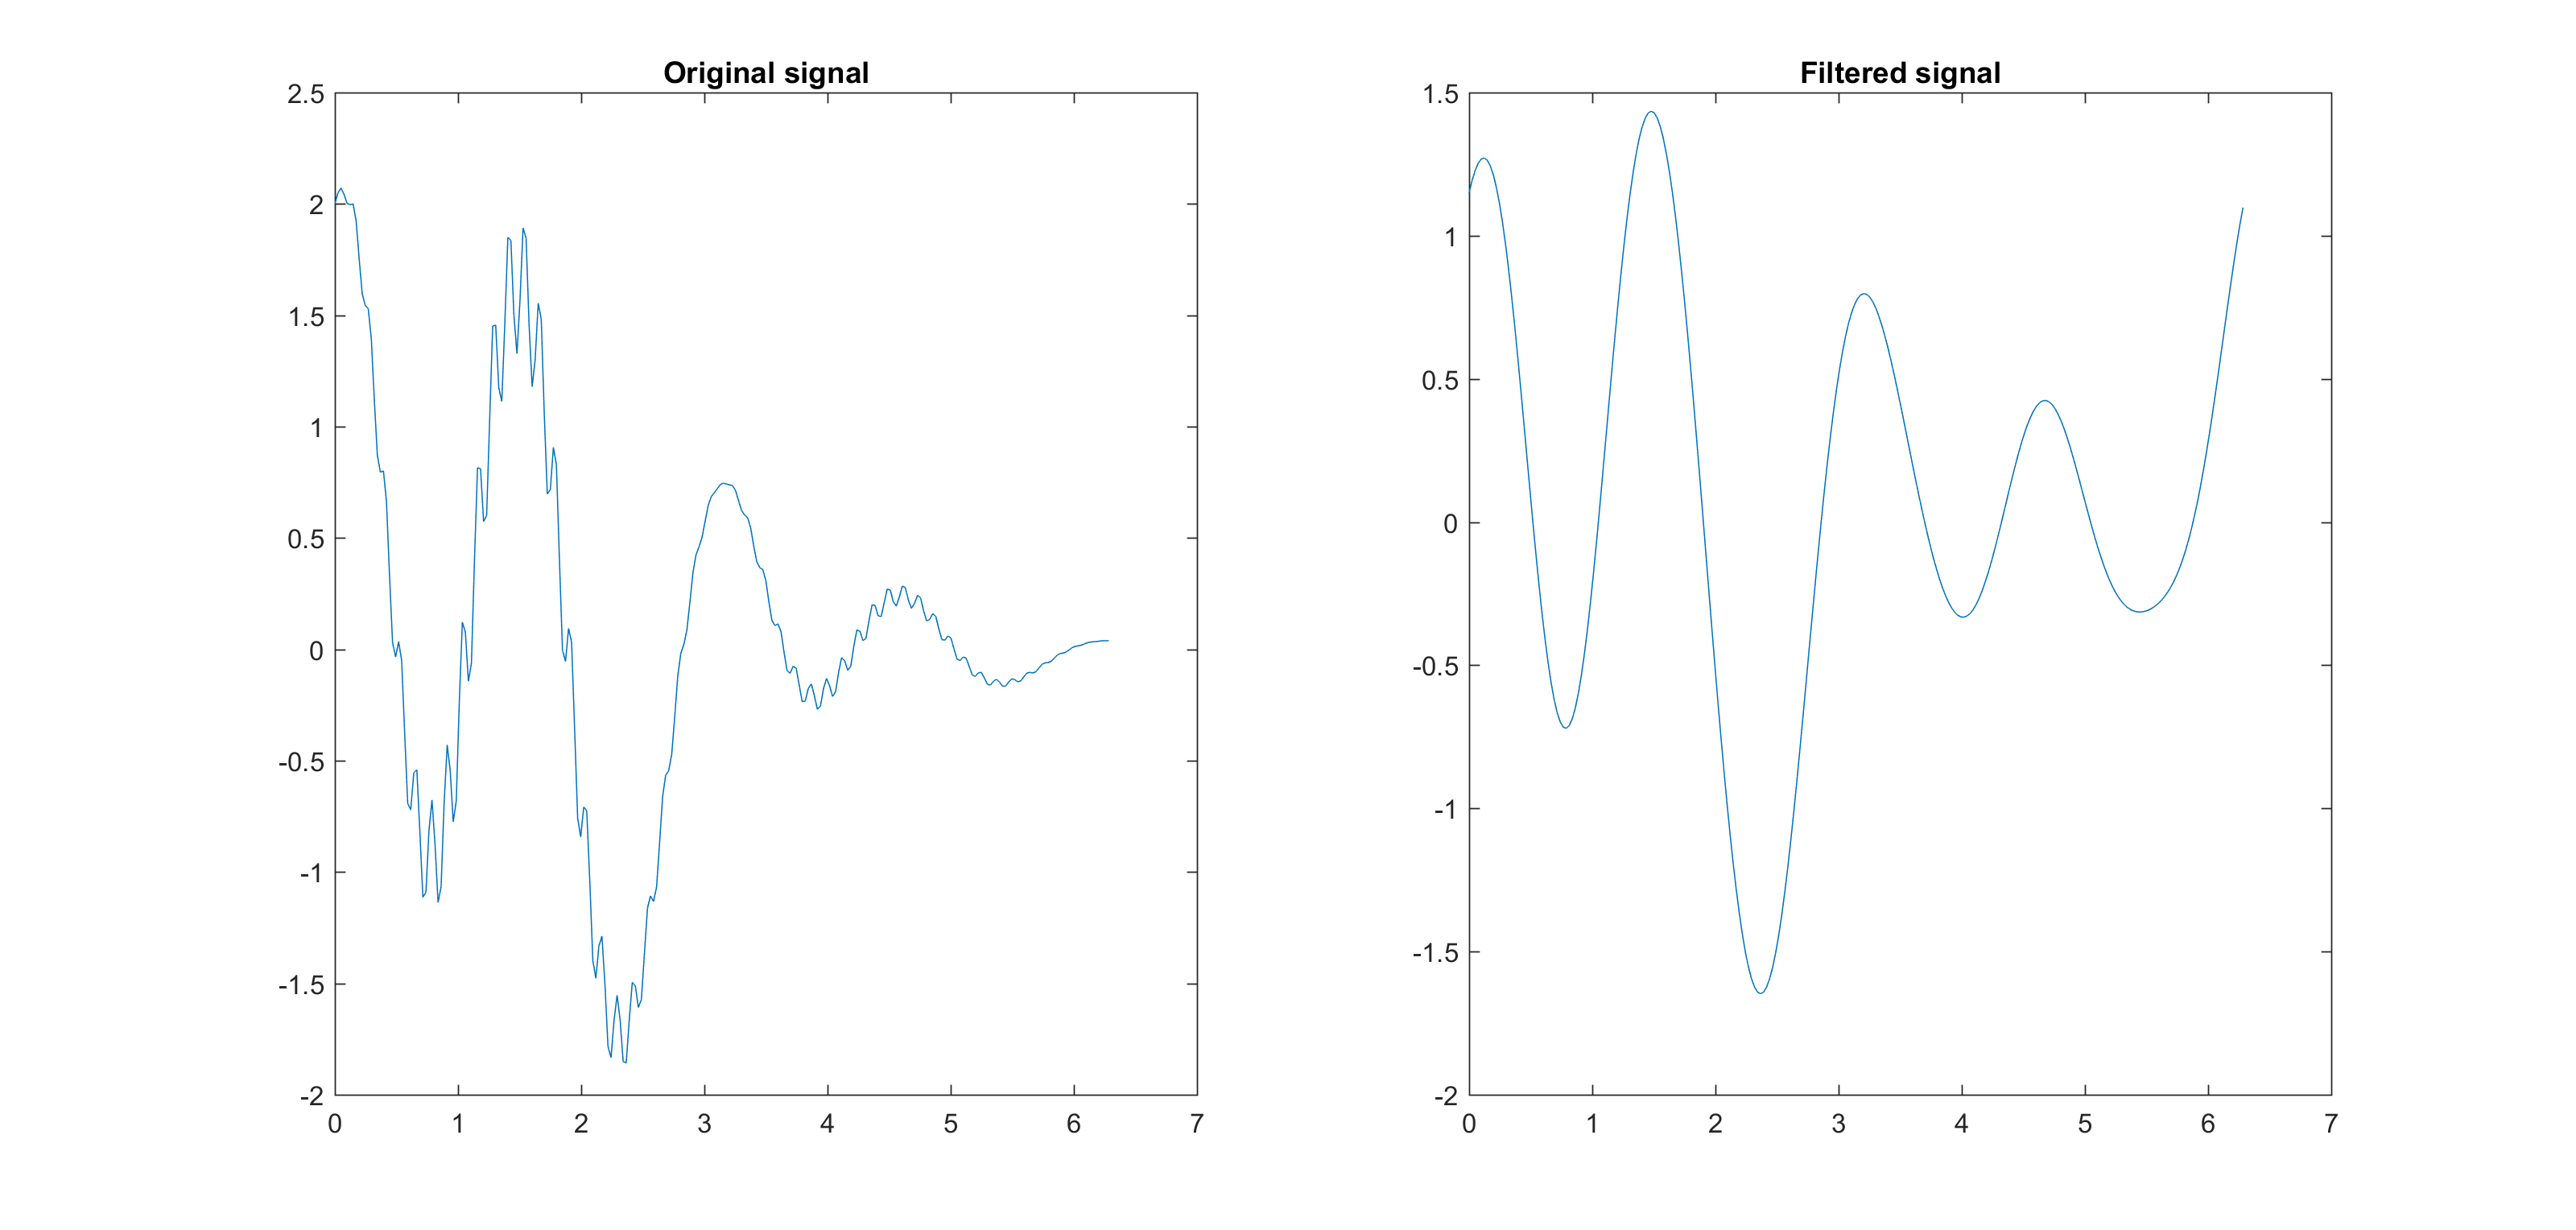
\includegraphics[width=6.5in]{Filter1.png}
% 	\caption{A signal and the result after a basic filter. The FFT was used to create the plot on the right.}
% \end{figure}

% \section{Section Test Example 3}
% Test section for toc display only.

% \begin{figure}[!h]
% 	\caption{There is nothing to see here.}
% \end{figure}

% \begin{figure}[!h]
% 	\caption{There is another float here. I wonder what could be here? Guess what? Nothing! There is no material in this float.}
% \end{figure}

% \subsection{Subsection Test 1}
% Test subsection for toc display only.

% \subsection{Subsection Test 2}
% Test subsection for toc display only.